\documentclass{article} %<<<
\usepackage{fancyvrb}
\usepackage{mathpazo}
\usepackage{microtype}
\usepackage{tikz}

\usepackage{hyperref}

\usetikzlibrary{automata,positioning,arrows}
\tikzset{automaton/.style={auto,node distance=1cm,on grid}}
\tikzset{every state/.style={minimum size=0pt,inner sep=1pt}}
\tikzset{transition/.style={->,>=stealth',shorten >=1pt}}
\tikzset{every initial by arrow/.style={transition}}
\tikzset{initial text={}}

\title{Static Checking of TOPL Properties}
\author{
  Dino Distefano
  \and Radu Grigore
  \and Rasmus Lerchedahl Petersen
  \and Nikos Tzevelekos}

%>>>
\begin{document} %>>>
\maketitle

We want to prove that a given program does not violate a given topl property.
The main idea is that almost any static analyzer is sufficient.
The details say how exactly to use a given static analyzer to check topl properties.
It seems desirable to have a couple of implementations.
One will be based on coreStar;
another could be based on something like Boogie.

Consider the topl property
\[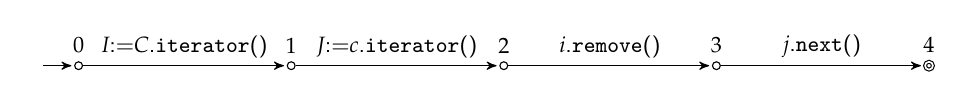
\begin{tikzpicture}[automaton,node distance=2.7cm]\footnotesize
  \node[state,initial] (q0) [label=above:$0$] {};
  \node[state] (q1) [label=above:$1$,right=of q0] {};
  \node[state] (q2) [label=above:$2$,right=of q1] {};
  \node[state] (q3) [label=above:$3$,right=of q2] {};
  \node[state,accepting] (q4) [label=above:$4$,right=of q3] {};
  \path[transition]
    (q0) edge node{{\it I}{\sf :=}{\it C}{\sf.}{\tt iterator}{\sf()}} (q1)
    (q1) edge node{{\it J}{\sf :=}{\it c}{\sf.}{\tt iterator}{\sf()}} (q2)
    (q2) edge node{{\it i}{\sf.}{\tt remove}{\sf()}} (q3)
    (q3) edge node{{\it j}{\sf .}{\tt next}{\sf()}} (q4);
\end{tikzpicture}\]
To check that a program does not violate it we run a static verifier on a modified program.
We add global variables {\tt state}, {\tt c}, {\tt i}, and~{\tt j}.
We replace calls to {\tt iterator} by calls to {\tt iterator'}, calls to {\tt remove} by calls to {\tt remove'}, and calls to {\tt next} by calls to {\tt next'}.
The primed methods are implemented as follows.
\begin{Verbatim}[fontsize=\footnotesize]
  Iterator iterator'() {
    emit(new Event(1, new Object[]{this}));
    Iterator r = iterator();
    emit(new Event(2, new Object[]{r}));
    return r;
  }
  void remove'() {
    emit(new Event(3, new Object[]{this}));
    remove();
    emit(new Event(4, new Object[0]));
  }
  Object next'() {
    emit(new Event(5, new Object[]{this}));
    Object r = next();
    emit(new Event(6, new Object[]{r}));
  }
\end{Verbatim}
This is essentially the same as is done in the runtime verifier---each observable method announces when it is called and when it returns.
Each call and each return gets an \emph{event identifier} (from~$1$ to~$6$ in this example).
Strictly speaking, events $4$~and~$6$ are not necessary.
In this example events carry $0$~or~$1$ objects, but for other properties there might be more, which is why an array is used to store them.
The method {\tt emit} is supposed to implement the semantics of an r-topl automaton.
\begin{Verbatim}[fontsize=\footnotesize]
  void emit(Event e) {
    Object c', i', j';
    events.enque(e);
    if (state == 0 && events.size() >= 2) {
      c' = c; i' = i; j' = j;
      i' = events[0].args[0];
      c' = events[1].args[0];
      state = 1;
      c = c'; i = i'; j = j';
      events.drop(2);
    } else if (state == 1 && events.size() >= 2) {
      c' = c; i' = i; j' = j;
      if (!(c' == events[0].args[0])) {
        events.drop(1); // skip
        return;
      }
      j' = events[1].args[0];
      state = 2;
      c = c'; i = i'; j = j';
      events.drop(2);
    } else if (state == 2 && events.size() >= 1) {
      c' = c; i' = i; j' = j;
      if (!(i' == events[0].args[0])) {
        events.drop(1); // skip
        return;
      }
      state = 3;
      c = c'; i = i'; j = j';
      events.drop(1);
    } else if (state == 3 && events.size() >= 1) {
      c' = c; i' = i; j' = j;
      if (!(j == events[0].args[0])) {
        events.drop(1); // skip
        return;
      }
      state = 4;
      c = c'; i = i'; j = j';
      events.drop(1);
    } else if (state == 4) events.drop(1); // skip
  }
\end{Verbatim}
In general there are multiple transitions outgoing from a state.
But, the idea is to infer a contract for this method and use it to verify the rest of the program.
Or, perhaps preferably, to generate the contract in the first place.
Now we find the contract by hand.
Two things must be clarified at this point:
\begin{enumerate}
\item what is the contract of the queue {\tt events}
\item the algorithm that generates the method {\tt emit}
\end{enumerate}

The queue {\tt events} has a fixed maximum size that is known in advance.
In fact, for topl properties the size is $0$,~$1$, or~$2$.

The method {\tt emit} switches on the {\tt state}.
If not enough events are available, then it only enqueues the current event.
Otherwise it tries each outgoing transition in turn.
If none matches, which is trivially true for {\tt state==4}, one event is skipped.
To try a transition, it makes a copy of variables {\tt c}, {\tt i}, and~{\tt j}, simulates each step, and if all matches it uses the (possibly updated) copies to overwrite the originals.


\end{document} %>>>
% vim:fmr=<<<,>>>:
